\chapter{Introduction}

Current debugging tools for robotics are mostly based on debugging techniques and interfaces developed for traditional non-robotic applications. Those techniques and interfaces were developed specifically to suit the requirements of traditional systems: First they assume that a program can be interrupted in its execution, which in a robotic environment is not possible most of the time. Second the data handled in traditional applications is usually discrete and based on user input, as opposed to the sensory data a robot handles. The data a robot handles is in general closely related to the real world environment of the robot and comes from sensors that provide a continuous data stream of readings. Although the computing world has changed in recent years, most tools have not. Robot developers often still use tools which were developed under different circumstances and based on different requirements. The application field of robotics has special requirements for debugging tools which are often not met by current debugging tools.

Traditional debugging tools usually render data collected during debugging as text and it's the developer's task to interpret the data. In a suspendable environment the developer has as much time as they need to interpret and analyse the data. When debugging robotic applications the developer usually has a lot less time, because of the nature of the application: Robotic applications usually can not be interrupted in their execution, because robots generally don't run in a deterministic and suspendable environment \cite{Gumbley2009}. Interrupting a robotic application would destroy the continuity in which the sensors collect data, the environment of the robot would change substantially and thus the robot's behaviour would change, which is an example of the ``probe effect'' and makes it hard to reproduce a fault unless it has a single cause \cite{Gumbley2009}. It is necessary to collect data during debugging without interrupting the execution of the program. Although some technical solutions have been presented in recent years \cite{Gumbley2009}, many developers still rely on printf-style debugging or other logging mechanisms. This approach is much simpler and does not require external tools, but the source code must be modified. Source code modification can be a problem with so called "Heisenbugs", software faults that disappear because the observation affected the bug \cite{Grottke2005}. The data collected with print or logging statements is usually text-only, which requires the developer to constantly parse and interpret logging messages. Due to the large amount of data that is processed this often means developer consoles are filled with logging messages that often contain more complex content such as numeric data.

ROSDashboard, the tool presented in this work, aims to support the developer during debugging by visualizing data in a graphic way and thus eliminating the cognitive effort needed to parse and interpret text based logging messages. While most of the currently available visualization tools in robotics focus on spatial data to help understand the robot and the environment in which it runs \cite{Collett2010, Quigley2009}, rendering of abstract data is still uncommon. ROSDashboard provides a dashboard interface to robot developers, which they can populate with graphical widgets to visualize all kinds of data from the robot. The dashboard can be customized to display widgets according to the current robot hardware and development stage. It can be used to visualize data during debugging as well as monitor data during the normal execution of the robot. This means ROSDashboard is a tool that a) can be adapted to many different use cases and b) allows the developer to choose the widgets he or she thinks represent the data best, according to their mental model and the meaning of the data. The tool is based on ROS (Robot Operating System) which abstracts from specific robot hardware and takes care of inter process communication \cite{Quigley2009}.

\section{Problem Statement}
\label{problem_statement}
[\textbf{problems with robotic software, many different environments, not interruptable, ...}]
Debugging robotic systems can prove to be much more complicated then normal software systems. 

\section{ROS}
The Robot Operating System (ROS) is an Open Source framework for complex robotic systems. The first work on ROS was done as part of the STanford Artificial Intelligence Robot (STAIR) in 2007 \cite{Quigley2007}. The original software library was called \emph{Switchyard} and had been developed at Stanford. Later the library was refined and generalized to also suit the requirements of the Personal Robot Program at Willow Garage\footnote{www.willowgarage.com} \cite{Quigley2009}. The resulting general framework has been released as Open Source \cite{Quigley2009} and this section gives a short overview over the most important principles in ROS.

\begin{figure}[ht]
\centering
\subfigure[Stanford's STAIR]{
	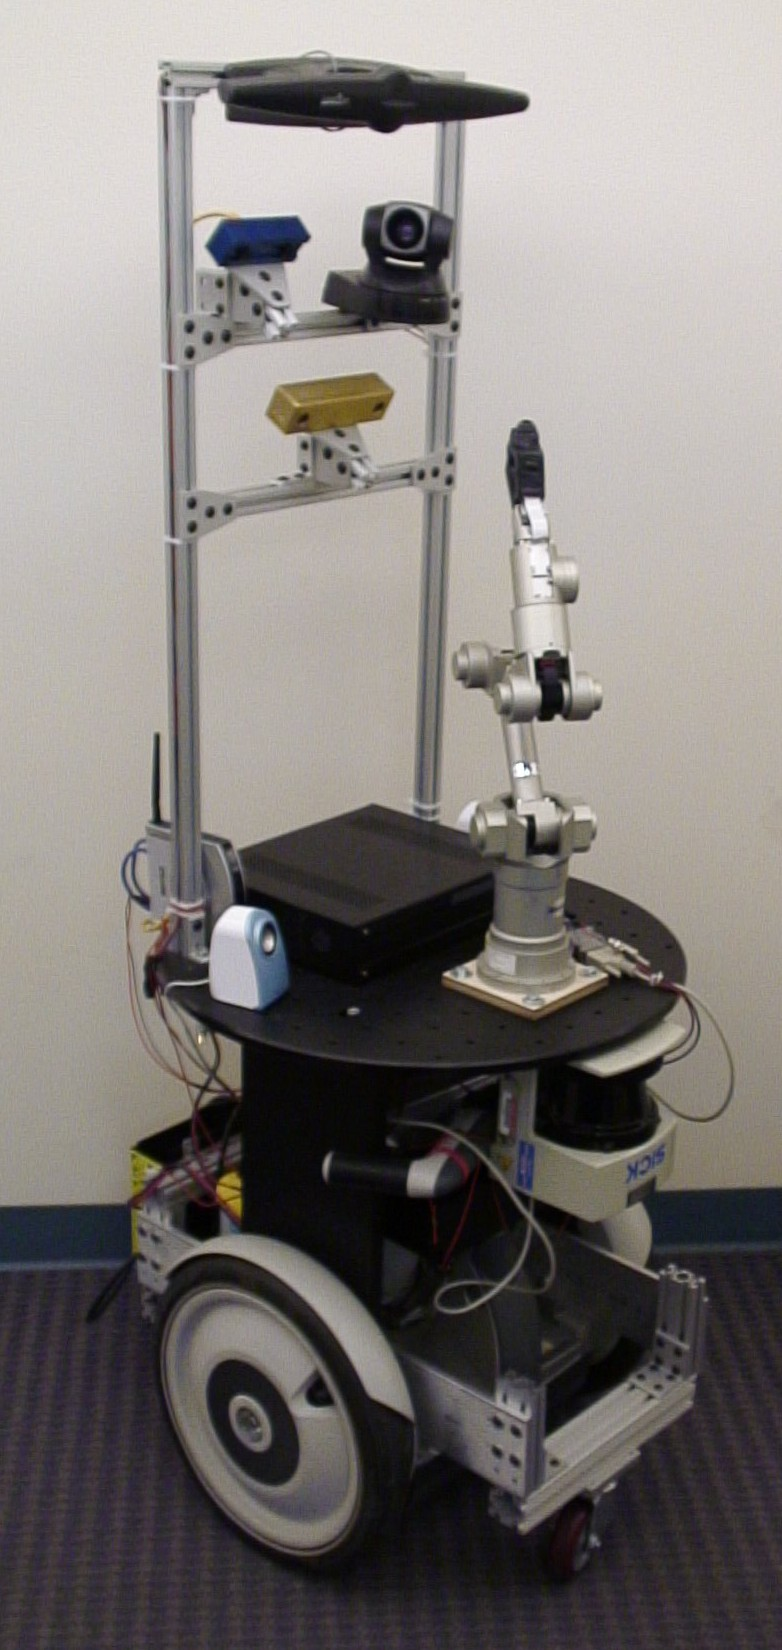
\includegraphics[height=8cm]{img/stair}
}
\subfigure[Willow Garage's PR2]{
	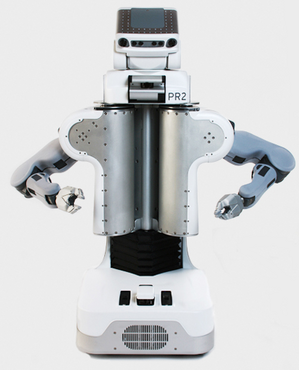
\includegraphics[height=8cm]{img/pr2}
}
\end{figure}

ROS was built to abstract from the hardware of the robot and create modular robot software, which can run on different robots and on different machines. This makes it easier to write software for robots and distribute the work to different teams, each team focusing on one part of the robot. The modules in ROS are called nodes and several nodes executed together are called a stack. ROS packages bundle nodes and stacks and are used to make software modules available to other developers. Everyone can create their own package which can be indexed by ROS so that your software modules can be found, downloaded and used by other developers. There exist many packages, nodes and stacks for some of the most common problems in robotics (e.g. navigation, localization, joint movement, etc.) and can easily be re-used.

The communication between ROS nodes can be done asynchronously through a publish/subscribe mechanism and synchronously through services. Nodes can send messages by publishing a message on a topic and receive messages by subscribing to that topic. This mechanism is really flexible and decouples the sender from the receiver. A publisher node does not need to know if there are other nodes listening and vice versa. For synchronous communication and guaranteed delivery of messages, services can be invoked. The routing is established during runtime through the ROS core. The core of ROS was kept really slim and only contains the most essential parts of the framework (such as the inter node communication). ROS can run on several machines distributed in a network, the only restriction is that every node needs to know the address of the core (master node) in order to communicate with other nodes.

\review

A variety of tools have been built around the ROS core to facilitate the development of ROS nodes and robotic software in general. They help you to create packages, nodes and stacks and execute and debug them. The philosophy for those tools is to be small and do one job only but do it good. This results in a really robust tools similar to the toolchain available on Linux. The downside is a big variety of tools in the ROS ecosystem, which can be confusing to new developers. See Section~\ref{related_ros_tools} for a more detailed analysis of current ROS tools.

The latest stable version of the ROS framework was released in April 2012 (ROS Fuerte). Previous releases of stable versions have been in August 2011 (ROS Electric), March 2011 (ROS Diamondback), August 2010 (ROS C Turtle) and March 2010 (ROS Box Turtle). There are currently many institutions, companies and individuals involved in the ROS community, contributing in many different ways. This makes ROS a god target platform, since we want to reach as many developers as possible (see Section~\ref{availability_developers}).

\section{Goals (?)}
Maybe it would be good to explain the goals of this work in the introduction: 

\section{Outline}
Explain all the chapters and sections of this work.
